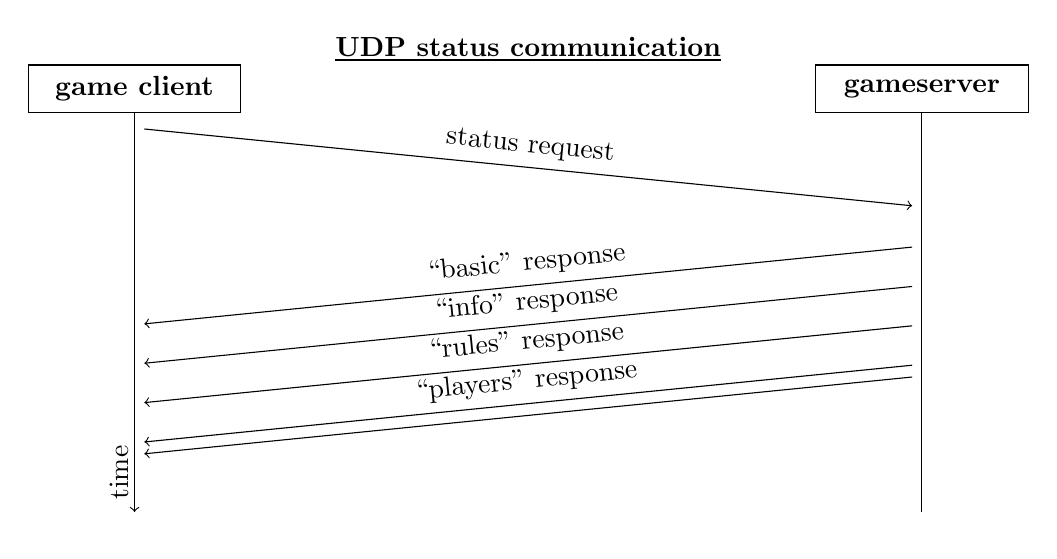
\begin{tikzpicture}

% figure title
\node[rectangle] at (5, 6) (title) {\underline{\bf UDP status communication}};

% game client and gameserver
\node[draw, rectangle, minimum height=0.6cm, minimum width=2.7cm] at ( 0, 5.5) (gctop) {\bf game client};
\node[draw, rectangle, minimum height=0.6cm, minimum width=2.7cm] at (10, 5.5) (gstop) {\bf gameserver};

% status
\node at ( 0,  5.0) (gcrq) {};
\node at (10,  4.0) (gsrq) {};
\draw[->] (gcrq) -- (gsrq) node[midway, above, sloped] {status request};

% basic
\node at (10,  3.5) (gsba) {};
\node at ( 0,  2.5) (gcba) {};
\draw[->] (gsba) -- (gcba) node[midway, above, sloped] {``basic'' response};

% info
\node at (10,  3.0) (gsin) {};
\node at ( 0,  2.0) (gcin) {};
\draw[->] (gsin) -- (gcin) node[midway, above, sloped] {``info'' response};

% rules
\node at (10,  2.5) (gsru) {};
\node at ( 0,  1.5) (gcru) {};
\draw[->] (gsru) -- (gcru) node[midway, above, sloped] {``rules'' response};

% players
\node at (10,  2.0) (gspl) {};
\node at ( 0,  1.0) (gcpl) {};
\draw[->] (gspl) -- (gcpl) node[midway, above, sloped] {``players'' response};

% multiple packets
\node at (10,  1.85) (gspl2) {};
\node at ( 0,  0.85) (gcpl2) {};
\draw[->] (gspl2) -- (gcpl2) {};


% gameserver and masterserver bottom, vertical lines
\node at ( 0, 0) (gcbot) {};
\node at (10, 0) (gsbot) {};
\draw[->] (gctop.270) -- (gcbot.90) node[at end, xshift=-0.2cm, yshift=0.5cm, rotate=90] {time};
\draw (gstop.270) -- (gsbot.90) {};

\end{tikzpicture}
